\documentclass[10pt]{article}
\usepackage[utf8]{inputenc}
\usepackage{graphicx}
\usepackage{float}

\title{Requirement Documentation}

\author{Team 3\\
        Shuying Chen, 400080161\\
        Ziyang Huang, 400051063\\
        Guiye Wu, 400089784
}
\date{Oct 6,2018}
\begin{document}
\maketitle
\newpage

 
\tableofcontents
\newpage

\section{Revision History}
\begin{table}[h!]
    \caption{Revision History: Requirement Documentation}
    \begin{center}
	\begin{tabular}{|p{2.5cm}|p{2.0cm}||p{2.0cm}|p{2.0cm}|}
	\hline
	\textbf{Developer} & \textbf{Date} & \textbf{Change} & \textbf{Revision}\\
	\hline
      Shuying Chen & Oct 5, 2018 & Initial Draft & 0\\
      \hline
      Ziyang Huang & Oct 5, 2018 & Initial Draft & 0\\
      \hline
      Guiye Wu & Oct 5, 2018 & Initial Draft & 0\\
      \hline
	\end{tabular}
    \end{center}
	\end{table}
	\newpage
\section{Project Drivers}
\subsection{The Purpose of the Project}
\subsubsection{The User Business or Background of the Project Effort}
This project is to redevelop a classic game minesweeper. The earliest minesweepers trace back to the 1960s, and this puzzle game style becomes popular during the 1980s. In modern time, minesweeper is the built-in game in window 7 system or the earlier version, for any other system it has to be downloaded in order to play this game. The game is very popular in earlier years, however, when the new systems are developed, the game is removed from the built-in games list and many people even don't know about the game nowadays. Our motivation is to renew this project and make it be well known.
\subsubsection{Goals of The Project}
The goal of this project is trying to redevelop the classic game -- minesweeper with a new style of the user interface with some funny features to increase the
enjoyment. This game is suitable for the users that would like practice logical thinking skills and being entertained at the same time. With different levels are included in this game, this will increase the playability for users from beginner to expert. The game will be re-implemented in python and can be easily accessed locally once it has been pre-downloaded on the computer. The advantage of this project is to provide our clients with a free-and-easy access minesweeper game whenever and wherever possible.
\subsection{The Stakeholders}
\subsubsection{The Client}
The client for our product will be the group of the general public that is interested in playing the new version of minesweeper game. They will also be the reviewer of the product. 
\subsubsection{The Customer}
The customer of the project will a group of the general public which is interested in consuming the game media. The entity, which members can be from all ages, who have the access and interact with our product will be the customer. 
\subsubsection{Other Stakeholders}
People, who have an interest in the game, either tangible or intangible, will be the other stakeholders for this software. 
This group of people may have different knowledge background for the game, so several levels of difficulties are provided, so this software will be suitable for the public and the basic tutorial is provided if needed.
\subsection{Mandated Constraints}
\subsubsection{Solution Constraints}
The product should re-size and re-allocate itself according to the different size of the dialogue box. The users can re-size the dialogue box as they wish, and the game should always be in the middle of the dialogue box and with the size of three-quarters of the dialogue box. \newline
Also, the project must be the re-implementation of the classic minesweeper game, which is an open-source project that was written in Java. We will need to implement a project wrote in python that has similar functionality as the classic minesweeper game.\newline

\subsubsection{Implementation Environment of the Current System}
The game will require the user to download ahead, and it will be a stand-alone game. The user can play the game locally on their computer.
\subsubsection{Partner of Collaborative Applications}
The product references to the classic Microsoft Minesweeper game, and the product is based on open source minesweeper codes which are written in Java.  Furthermore, the product will be written in Python and pygame will be the collaborative application.
\subsubsection{Off-the-Shelf Software}
For the product to be executed the following off-the-shelf software is required:\\\\
a)Python(available from https://www.python.org)\\
\\
b)A client where the interface can run
\subsubsection{Anticipated Work-space Environment}
The anticipated workplace environment for the product is anywhere. It can be played at any time, anywhere as you want, as long as you have the game downloaded before. It is an off-line application.
\subsubsection{Schedule Constraints}
The is no such a schedule constraint for our team. The basic deadline is about the beginning of December when we need to present our project.
\subsubsection{Budget Constraints}
The budget for the whole project is $\$0$.
\subsubsection{Enterprise Constraints}
The game can be downloaded to local and it is free and easy to play, only with some logic.
\subsection{Naming Conventions and Terminology}
\begin{itemize}
    \item Functional Requirement: Describe what services the software-to-be should provide
    \item Non-function Requirement: Constrain how such services should be provided
    \item Client: The group of people will provide their expectations on the product.
    \item Consumer: The group of people who are trying to be satisfied. They will be the entity that will consume the final product.
    \item Stakeholder: A person, group or organization that has interest or concern in the success of the project.
    \item User: The person who will eventually use the final product.
    \item  Minesweeper: The name of the classic game, which we will re-implement on
\end{itemize}
\subsection{Relevant Facts and Assumptions}
\subsubsection{Relevant Facts}
The relevant fact is that the original implementation of this game contains about 1200 lines of code, and it needs to run on a web browser.
\subsubsection{Business Rules}
We need to work together at the same time like in the office and try to make the same effort for this project.
\subsubsection{Assumptions}
The project is developed for a single user, it can be run on a laptop or computer at any location because it is offline software. The project is not a large software, it does not have any requirements on CPU or memory for modern computers.
\section{Functional Requirements}
\subsection{The Scope of The Work and the Product}
\subsubsection{The Context of The Work}
Deliverable
	\begin{itemize}
		\item Required Documentation
		\item Final Software
	\end{itemize}
	Deadlines
	\begin{itemize}
		\item Requirements Document Revision 0:  October 06
		\item Proof of Concept Demonstration:			October 16
		\item Functioning Prototype: 			October 20
		\item Automated Testing prototype:       October 21
		\item Test Plan Revision 0:        		October 27
		\item Design Documentation:				November 10
		\item User documentation:				November 17
		\item Test Report Revision 0:			November 27
		\item Functioning Program:				
		November 27
		\item Final Documentation:				December 6
	\end{itemize}
\subsubsection{Work Partitioning}
\begin{table}[h!]
    \caption{Work Partitioning}
    \begin{center}
	\begin{tabular}{|p{2.0cm}|p{2.0cm}|p{3.0cm}|p{2.5cm}|}
	\hline
	\textbf{Event numner} & \textbf{Event Name} & \textbf{Input} & \textbf{Output}\\
	\hline
      1 & Minesweeper Game Board & Code & User Interface\\
      \hline
      2 & Minesweeper Graphic & Code and Graphics & User Interface \\
      \hline
      3 & Minesweeper Rules & Code & User Interface\\
      \hline
      4 & Minesweeper Audio Effects &  Microphone & Audio Output Device\\
      \hline
      5 & Minesweeper Final Edit & Code & User Interface \\
      \hline
	\end{tabular}
    \end{center}
	\end{table}
\newpage
\subsubsection{Individual Product Use Cases}
    \begin{figure}[ht!]
    \centering
    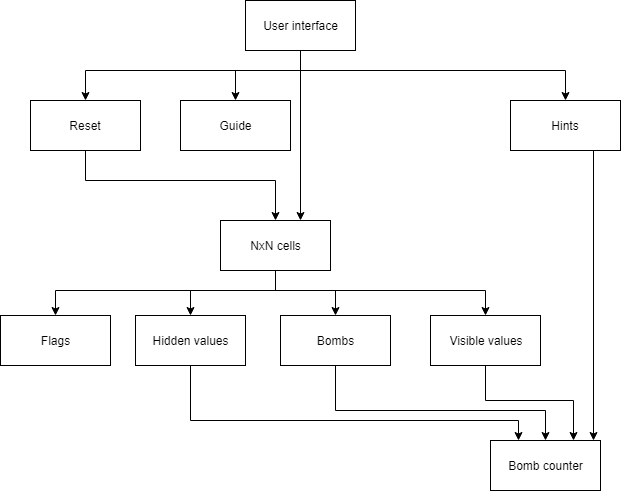
\includegraphics[width=100mm]{UseCases.png}
    \caption{UseCases}
    \label{fig1:Use Cases}
    \end{figure}
    \begin{figure}[ht!]
    \centering
    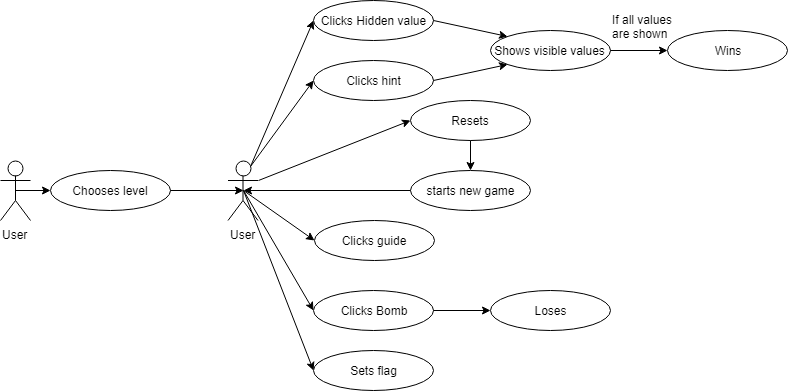
\includegraphics[width=100mm]{UseCasesDiagram.png}
    \caption{UseCasesDiagram}
    \label{fig1:Use Cases}
    \end{figure}
    
\subsection{Functional Requirements}
\subsubsection{Input}
\begin{enumerate}

    \item The software is able to read user's position of clicking blocks and record the coordinate for other functional operations.
    \item Left clicks on the cell will be considered as visualizing the hidden values
    \item Right clicks on the cell will be considered as setting flags
    \item Click the icon above the playing area will be considered as an input.


\subsubsection{Output}
    \item If the player clicks a non-block, the block will either show the blank space of corresponding numbers.
    \item If the player clicks a bomb, the block will show the icon of the bomb and terminate the game.
    \item If the player right-lick the mouse on to the blocks, the will be a "flag" shown on the blocks that the block is being tagged.
    \item If the player click the icon above the playing area, the current game will clear out and a new game is restarted.


\subsubsection{Other functional Requirements}

\item The game has a convenient button for the user to click, which will show all the number around the clicked cell, if the neighboured bombs are flagged right.
\item The game has three difficult levels that are easy, normal and hard. The easy model is 10 times 10 cells, the normal model is 20 time 30 cells and the hard model is 40 times 60 cells.
\item The game can be reset during any condition of the game.
\item The game is over when user hits the bomb.
\item The game is passed when user finds out all the hidden values on the board.
\item The hidden values on the board will convert to visible values when the values are clicked.
\item All the cells and the reset button are clickable on the board.
\item The game provides 'flag' that allows user to put on the board to indicate a bomb.
\end{enumerate}
\section{Non Functional Requirements}
\subsection{Look and Feel Requirements}
\begin{enumerate}
\item The game interface shall looks comfortable according to the funny features

\subsection{Usability and Humanity Requirements}

\item The software shall be easy to use for people older than 5 years.
\item The game provides guide for new players, and the guide contains all the game rules in details.

\subsection{Performance Requirements}
\subsubsection{Speed Requirements}

\item The response time of the system should be fast.
\item Setting up a new game should be fast.

\subsubsection{Safety Critical Requirements}

\item The software shall not make any injures on user.

\subsubsection{Reliability and Availability Requirements}

\item The software can be run any time and it will be usable for 24 hours per day, 365 days or 366 days per year.

\subsubsection{Precision Requirements}

\item Each cell contains either value or bomb.
\item The size of the value, bomb and flag should fit to the size of each cell.
\item The reset button, the guide button and each cell are large enough to be clicked.
\item The values shall be clear to recognize.
\item The location of value, bomb and flag should be aligned to the cell position.

\subsubsection{Capacity Requirements}

\item The software takes less than 10 mb memory to be downloaded.

\subsection{Operational and Environmental Requirements}
\subsubsection{Excepted Physical Environment}
\item The software is used when user clicks the game icon and chooses a difficult level.
\subsubsection{Excepted Technological Environment}
\item The software can only be used after downloading.
\subsection{Maintainability and Support Requirements}
\subsubsection{Maintainability}

\item The software can run without internet.

\subsubsection{Portability}

\item The software is expected to run on Windows, Linux and Mac environments.

\subsection{Security Requirements}

\item The software does not require any information from the user.\\
\item  The software will not read or destroy or execute any data from the local machine.

\subsection{Cultural Requirements}

\item The software does not include any feature that offends user's culture.

\subsection{Legal Requirements}

\item The software is redevelopment from a open-source code.

\subsection{Health and Safety Requirements}

\item The software shall not make any injures on user.
\end{enumerate}
\section{Project Issues}
\subsection{Open Issues}
N/A
\subsection{Off-the-shelf Solutions}
\subsubsection{Ready-Made Products}
\begin{itemize}
    \item Interface
\end{itemize}
\subsubsection{Reusable Components}
Modularized code components
\subsubsection{Products That Can Be Copied}
The original code cannot be copied, but it can be a reference and a prototype that we can rely on.
\subsection{New Problems}
\subsubsection{Effects on the Current Environment}
The new product will be an off-line user interfaced game. It will be played locally without any interrupting of the laptop. It is really safe and stable.
\subsubsection{Effects on the Installed Systems}
There is an interface along with the system.

\subsubsection{Potential User Problems}
Some potential users who do not know the rules and logic may be a headache about the game and very stressful.

\subsubsection{Limitations in the Anticipated Implementation Environment That May Inhibit the New Product}
The server that will host our product will not be powerful enough to hold the desired amount of users with our project growth pattern.
\subsubsection{Follow-Up Problems}
The will be no follow-up problems that we take together, make the same effort to the program.
\newpage
\subsection{Tasks}
\subsubsection{Project Planning}
\begin{table}[ht!]
    \caption{Project planning}
    \begin{center}
	\begin{tabular}{|p{2.5cm}|p{2.0cm}|p{2.0cm}|}
	\hline
	\textbf{Task} & \textbf{Roles of Completes} & \textbf{Time}\\
	\hline
      Model Implementation & Software Engineers & OCT 15\\
      \hline
      Model Revision & Client & OCT 26\\
      \hline
      Python Design & Software Engineers & NOV 9\\
      \hline
      Interface Implementation & Software Engineers & NOV 15\\
      \hline
      Revision & Client & NOV 23\\
      \hline
      Publishing & Software Engineers & NOV 26\\
      \hline
	\end{tabular}
    \end{center}
	\end{table}
\subsection{Migration to the New Product}
None.
\subsection{Risks}
There is no risk for this project.
\subsection{Costs}
There is no cost for this project.
\section{User Documentation and Training}
\subsection{Waiting Room}
Additional functionality of the game functionality and visual as well as audio effects.
\subsection{Ideas for Solutions}
Proper hierarchy and documentation of python code.
\section{Appendix}
\subsection{Symbolic Parameters}
N/A
\end{document}